\section{Introduction}
\begin{frame}{Cellular Automata}
     \small
\begin{columns}

    \column{0.6\textwidth}
     \begin{itemize}

    \item \textit{Automaton} (plural: \textit{automata}) is a term used in for a theoretical machine that changes its internal state based on inputs and its previous state. 

         \item The state set is usually defined as finite and discrete, which often causes nonlinearity in the system’s dynamics

     \item \textit{Cellular automata} are a set of such automata arranged in a regular spatial grid, whose states are simultaneously updated by a uniformly applied state-transition function that refers to the states of their neighbors.
     \end{itemize}
     \column{0.4\textwidth}
     \begin{center}
         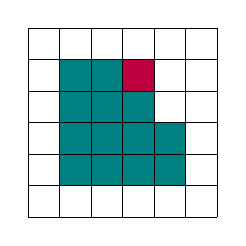
\begin{tikzpicture}[scale=0.4]
        \fill (1,1)[teal] rectangle (4,5);
        \fill (1,1)[teal] rectangle (5,3);
        \fill (3,4)[purple] rectangle (4,5);
        \draw[black] (0,0) grid (6,6);
    \end{tikzpicture}

    Example of cellular automata for modelling forrest fire. Green represents trees, white space empty space, and red starting fire.
     \end{center}
     
\end{columns}
    

    


\end{frame}

\begin{frame}
\frametitle{Introduction cellular automata}
     \small
\begin{itemize}
    \item \textbf{Definition:} Cellular automata (CA) are discrete, computational models used to simulate complex systems and processes. They consist of a grid of cells, each in one of a finite number of states, updating simultaneously according to a set of local rules.
    \item \textbf{History and Origin:}
    \begin{itemize}
        \item Introduced by mathematicians Stanislaw Ulam and John von Neumann.
        \item Initially conceptualized as a mathematical abstraction for self-replication.
    \end{itemize}
    \item \textbf{Characteristics:}
    \begin{itemize}
    \scriptsize
        \item \textbf{Grid:} Usually 2D, but can be 1D or 3D.
        \item \textbf{States:} Common examples include binary states (0 and 1) but can be more complex.
        \item \textbf{Neighborhoods:} Typically include adjacent cells (e.g., Moore or von Neumann neighborhoods).
        \item \textbf{Rules:} Simple local interactions that determine the state of a cell in the next generation.
    \end{itemize}
   
\end{itemize}
\end{frame}


\begin{frame}{Significance}
    \begin{itemize}
        \item Demonstrates how complex patterns and behaviors can emerge from simple rules applied at local levels.
        \item Used as a theoretical tool to study self-organization in natural systems.
    \end{itemize}
    
\end{frame}

\begin{frame}{John von Neumann}
\small
John von Neumann (1903–1957): Hungarian-American polymath  made pioneering contributions across multiple scientific disciplines. 
    \begin{columns}
    \column{0.2\textwidth}
            \includegraphics[width=\textwidth]{lesson_4/images/von_neumann.jpg} 
            
    \column{0.8\textwidth}
            \scriptsize
            
            \begin{itemize}
                \item \textbf{Mathematics:} significant contributions to set theory, functional analysis, and the foundations of mathematics.
                \item \textbf{Quantum Mechanics:}  mathematical formulation of quantum mechanics, the axiomatic Hilbert space framework.
                \item \textbf{Computer Science:} Developed the Von Neumann architecture, the basis for most modern computer designs.
                \item \textbf{Game Theory:} founder of game theory, co-authored "Theory of Games and Economic Behavior," .
                \item \textbf{Nuclear Physics:} Played a key role in the Manhattan Project and  in the development of the hydrogen bomb.
                \item \textbf{Statistics and Economics:} profoundly influenced economic theories .
                \item \textbf{Cellular Automata:} Proposed a self-replicating machine model using cellular automata,  foundation for the field of artificial life.
            \end{itemize}

        
    \end{columns}
\end{frame}

\begin{frame}{Example of patter evolution}
    \begin{itemize}
        \item The initial pattern constitutes the first generation of the system. 
        \item The second generation is created by applying the above rules simultaneously to every cell in the first generation in parallel-- births and deaths happen simultaneously. 
        \item The rules continue to be applied repeatedly to create further generations.
        \item The rules determine the new states of each of the cells inp from the states of that cells and its neighbours
        \item The size of neighbourhoods determine the extent of the interaction between cells in the grid
    \end{itemize}
\end{frame}

\begin{frame}{Properties of Cellular Automata}
Important properties which distinguis Cellular automata
\begin{itemize}
    \item \textbf{Localism:} States are updated based on the properties of the neighbourhood
    \item \textbf{Parallelism:} The state of every cell is updated in parallel
    \item \textbf{Homogeneity:} The same set of rules is applied across the automaton
\end{itemize}
\begin{center}
   These properties distinguish cellular automata from other types of automata or algorithm. 
\end{center}


\end{frame}



\begin{frame}{Properties of Cellular Automata}
\begin{itemize}
    \item It is \textbf{impossible} to predict, in advance, what behavior will be displayed by the Cellular Automata given a set of rules.
    \item There are a number of possible states into which a CA can descend into
    \item Stephen  Wolfram proposed a classification scheme based on these criteria:
    \begin{itemize}
        \item Evolution leads to a homogeneous state. 
    \item Evolution leads to a set of separated simple stable or periodic structures. 
    \item Evolution leads to a chaotic pattern. 
    \item Evolution leads to complex localized structures, sometimes long-lived.
    \end{itemize}

\end{itemize}
\end{frame}

\begin{frame}{Applications of Cellular Automata}

    \only<1>{
        \textbf{Simulation of Fluids:} Cellular automata are used to model fluid dynamics by discretizing the fluid space and applying rules for the interaction of particles, mimicking the behavior of real fluids.
        \vfill
        \begin{center}
            \includegraphics[width=\textwidth]{lesson_4/images/ca_fluid.png}
        \end{center}
    }
    \only<2>{
       \textbf{Epidemic Models:} Cellular automata help simulate the spread of diseases by modeling individuals as cells and defining rules for infection transmission and recovery.
        \vfill
        \begin{center}
            \includegraphics[scale=0.3]{lesson_4/images/ca_epidemics.jpeg}
        \end{center}
    }
    \only<3>{
        \textbf{Simulation of Cancer Cell Growth:} Cellular automata model the proliferation of cancer cells and their interactions with the surrounding tissue to understand and predict growth patterns.
        \vfill
        \begin{center}
            \includegraphics[scale=0.12]{lesson_4/images/ca_tumor.png}
            \includegraphics[scale=0.4]{lesson_4/images/ca_tumor_2.jpg}
        \end{center}
    }
    \only<4>{
       \textbf{Art and design:} Some artists experiments cellular automata to create complex, evolving patterns and textures that are used in digital art and visual effects.
       \vfill
       \begin{center}
           \includegraphics[scale=0.25]{lesson_4/images/ca_art.jpg}
       \end{center}
    }
    \only<5>{
       \textbf{Art and design:} Cellular automata were also used for visual effect in Noita game
        \vfill
        \begin{center}
            \includegraphics[scale=0.3]{lesson_4/images/ca_noita.jpg}
        \end{center}
    }
    \only<6>{
        \textbf{Simulation of Forest Fires:} Cellular automata model the spread of fire through a forest based on wind, vegetation, and other factors, useful in understanding and managing wildfires.
        \vfill
        \begin{center}
            \includegraphics[scale=0.2]{lesson_4/images/ca_fire.png}
        \end{center}
    }
    \only<7>{
       \textbf{Simulations of Social Movements:} These models use cellular automata to represent social dynamics and group behaviors, aiding in the study of phenomena like crowd movements and protests.
        \vfill
        \begin{center}
            \includegraphics[scale=0.6]{lesson_4/images/ca_crowd.png}
        \end{center}
    }
\end{frame}



